%% Relatorio do TP2 -- formato AAAI.
%% Preambulo copiado do template oficial da AAAI (Overleaf). Se o seu template
%% for de outro ano (ex.: aaai25), troque so o nome do pacote na linha 2.
\documentclass[letterpaper]{article} % DO NOT CHANGE THIS
\usepackage{aaai2026}  % DO NOT CHANGE THIS (sem [submission]: mostra o autor)
\usepackage{times}  % DO NOT CHANGE THIS
\usepackage{helvet}  % DO NOT CHANGE THIS
\usepackage{courier}  % DO NOT CHANGE THIS
\usepackage[hyphens]{url}  % DO NOT CHANGE THIS
\usepackage{graphicx} % DO NOT CHANGE THIS
\urlstyle{rm} % DO NOT CHANGE THIS
\def\UrlFont{\rm}  % DO NOT CHANGE THIS
\usepackage{natbib}  % DO NOT CHANGE THIS AND DO NOT ADD ANY OPTIONS TO IT
\usepackage{caption} % DO NOT CHANGE THIS AND DO NOT ADD ANY OPTIONS TO IT
\frenchspacing  % DO NOT CHANGE THIS
\setlength{\pdfpagewidth}{8.5in} % DO NOT CHANGE THIS
\setlength{\pdfpageheight}{11in} % DO NOT CHANGE THIS

% Pacotes adicionais (permitidos pelo template)
\usepackage[brazilian]{babel}
\usepackage{booktabs}

\pdfinfo{
/TemplateVersion (2026.1)
}

\setcounter{secnumdepth}{0} % DO NOT CHANGE THIS

% unidades de tempo
\newcommand{\ns}{\,ns}
\newcommand{\us}{\,$\mu$s}
\newcommand{\ms}{\,ms}

\title{A Consultoria do Blibblon: \'Indice de Clientes em \'Arvore AVL e Tabela Hash,\\
Fila de Prioridade e Conjuntos Disjuntos}

\author{
    Andr\'e Rafael Batista
}
\affiliations{
    Departamento de Ci\^encia da Computa\c{c}\~ao\\
    Universidade Federal de Minas Gerais (UFMG)\\
    Belo Horizonte, MG, Brasil\\
    andrerafaelbatista@dcc.ufmg.br
}

\begin{document}

\maketitle

%% =====================================================================
\begin{abstract}
Este trabalho implementa o sistema da Consultoria do Blibblon, que cadastra clientes e regi\~oes, responde buscas por poder exato e por faixa de poder, atende clientes por prioridade e informa se duas regi\~oes est\~ao conectadas. O \'indice de clientes pode alternar, durante a execu\c{c}\~ao, entre uma \'arvore AVL com chave composta (poder, identificador) e uma tabela hash com encadeamento separado e fun\c{c}\~ao multiplicativa de Fibonacci, preservando o estado l\'ogico. A fila de atendimento \'e um heap bin\'ario de m\'aximo e a conectividade \'e mantida por conjuntos disjuntos com compress\~ao de caminho e uni\~ao por posto. A an\'alise experimental, com at\'e $10^6$ clientes e $10^5$ regi\~oes, mostra que a hash \'e de 2,5 a 15 vezes mais r\'apida nas opera\c{c}\~oes pontuais, enquanto a AVL \'e de 33 a 76 vezes mais r\'apida na busca por faixa (at\'e 4400 vezes em faixas estreitas). A remo\c{c}\~ao \'e a opera\c{c}\~ao que mais diverge: com muitos clientes por poder, ela fica 23 vezes mais lenta na hash, enquanto a AVL n\~ao \'e afetada. Os conjuntos disjuntos respondem conectividade em cerca de 10\ns, contra at\'e 14\ms\ de uma busca em largura.
\end{abstract}

%% =====================================================================
\section{Introdu\c{c}\~ao}

A Consultoria Trombaferro recebe aventureiros com builds prontas e precisa responder tr\^es tipos de pergunta: quem s\~ao os clientes com um poder espec\'ifico ou dentro de uma faixa de poder, quem deve ser atendido em seguida, e se \'e poss\'ivel ir de uma regi\~ao a outra do mapa. O sistema processa uma sequ\^encia de comandos lidos da entrada padr\~ao: troca do modo do \'indice (\texttt{E}), cadastro de atributo (\texttt{A}), de cliente (\texttt{C}), de regi\~ao (\texttt{R}) e de rota (\texttt{T}), encerramento de cliente (\texttt{D}), busca por poder exato (\texttt{BP}) e por faixa (\texttt{BF}), consulta de conectividade (\texttt{CC}), entrada na fila (\texttt{F}) e atendimento (\texttt{Z}).

Diferentemente do TP1, em que uma estrutura central respondia por quase tudo, aqui cada pergunta tem uma estrutura adequada, e o desafio central \'e o \'indice de clientes, que precisa funcionar com duas estruturas internas de caracter\'isticas opostas. Uma \'arvore de busca balanceada mant\'em as chaves ordenadas e favorece consultas por faixa. Uma tabela hash oferece acesso pontual em tempo esperado constante, mas n\~ao preserva ordem alguma. O sistema deve permitir a migra\c{c}\~ao entre as duas a qualquer momento, sem alterar nenhuma resposta. Os outros desafios s\~ao atender sempre o cliente de maior prioridade, com desempate pelo menor identificador, enquanto entradas e atendimentos se intercalam, e responder conectividade num mapa que s\'o cresce.

A solu\c{c}\~ao usa seis TADs: \texttt{Atributo}, \texttt{Cliente}, \texttt{Indice} (fachada sobre \texttt{ArvoreAVL} e \texttt{TabelaHash}), \texttt{Mapa}, \texttt{FilaPrioridade} e \texttt{ConjuntosDisjuntos}, todos implementados sem a biblioteca de cont\^eineres do C++, sobre um vetor din\^amico pr\'oprio. O restante do artigo apresenta as fontes de apoio, as decis\~oes de projeto, a an\'alise de complexidade e uma avalia\c{c}\~ao experimental com cinco experimentos que comparam as estruturas sob diferentes cargas, incluindo uma discuss\~ao de localidade de refer\^encia.

%% =====================================================================
\section{Trabalhos Relacionados}

As estruturas cl\'assicas usadas aqui seguem principalmente \citet{cormen2009} e \citet{ziviani2011}. A \'arvore AVL foi proposta por \citet{adelson1962}; sua altura \'e limitada por cerca de $1{,}44\log_2 n$, e as quatro rota\c{c}\~oes de rebalanceamento seguem a apresenta\c{c}\~ao de \citet{ziviani2011}. Para a tabela hash, a escolha da fun\c{c}\~ao de espalhamento multiplicativa, e da constante derivada da raz\~ao \'aurea, segue \citet[Se\c{c}.~6.4]{knuth1998}, que tamb\'em analisa o comprimento esperado das listas no encadeamento separado. O heap bin\'ario vem de \citet{williams1964}, e a an\'alise dos conjuntos disjuntos com compress\~ao de caminho e uni\~ao por posto, de custo amortizado $O(\alpha(n))$, \'e de \citet{tarjan1975}.

Na an\'alise experimental, o modelo de grafos aleat\'orios de \citet{erdos1960} explica o surgimento de um componente gigante quando o grau m\'edio passa de 1, o que determina o custo da busca em largura. A discuss\~ao de localidade de refer\^encia se apoia em \citet{drepper2007}, e o gerador pseudoaleat\'orio usado nas cargas \'e o SplitMix64 de \citet{steele2014}.

%% =====================================================================
\section{M\'etodos}

O programa foi implementado em C++11 e compilado com \texttt{g++ -O2}. Todas as cole\c{c}\~oes usam um vetor din\^amico pr\'oprio (\texttt{lib::vetor}), que dobra a capacidade quando enche e verifica os \'indices com asser\c{c}\~oes. O programa principal l\^e os comandos da entrada padr\~ao, despacha cada um para os TADs e imprime a sa\'ida.

\subsection{Atributo e Cliente}

O \texttt{Atributo} guarda identificador e nome. O \texttt{Cliente} guarda identificador, nome, build (um valor por atributo cadastrado at\'e o momento) e poder, calculado uma \'unica vez no construtor como a soma da build. No comando \texttt{C}, a build come\c{c}a com zeros e cada par atributo-valor sobrescreve a posi\c{c}\~ao correspondente, de modo que, se um atributo se repete, vale o \'ultimo valor. O poder \'e armazenado em \texttt{long long}, porque a soma de muitos atributos pode exceder 32 bits, e pode ser negativo. Os clientes ficam num vetor de ponteiros indexado pelo identificador, o que permite que \texttt{D} encontre o cliente (e seu poder) em $O(1)$ antes de remov\^e-lo do \'indice.

\subsection{\'Indice: modo A (\'arvore AVL)}

Cada n\'o da AVL guarda um \'unico cliente, e a chave \'e o par (poder, identificador), comparado lexicograficamente. Essa decis\~ao tem tr\^es consequ\^encias. Primeiro, todas as chaves s\~ao distintas, ent\~ao a \'arvore n\~ao precisa de listas dentro dos n\'os e a remo\c{c}\~ao de um cliente custa $O(\log n)$, independentemente de quantos outros clientes tenham o mesmo poder. Segundo, o percurso em ordem produz exatamente a ordem exigida pela \texttt{BF}: poder crescente, com desempate por identificador crescente. Terceiro, a \texttt{BP} \'e simplesmente a faixa $[p, p]$, e os clientes saem automaticamente em ordem de identificador.

A inser\c{c}\~ao e a remo\c{c}\~ao s\~ao recursivas e, na volta da recurs\~ao, cada n\'o do caminho tem sua altura atualizada e \'e rebalanceado se o fator de balanceamento chegar a $\pm2$, com rota\c{c}\~ao simples ou dupla. Na remo\c{c}\~ao de um n\'o com dois filhos, o sucessor (o menor da sub\'arvore direita) \'e desligado da sub\'arvore, j\'a rebalanceada, e religado no lugar do n\'o removido. Os n\'os s\~ao reaproveitados, e nenhum dado \'e copiado entre eles. A busca por faixa \'e um percurso em ordem com poda: s\'o desce \`a esquerda se ainda pode haver poder $\ge min$, e s\'o desce \`a direita se ainda pode haver poder $\le max$.

\subsection{\'Indice: modo H (tabela hash)}

A tabela usa encadeamento separado, e cada entrada da lista de um balde representa um \emph{poder distinto}, com o vetor ordenado dos identificadores dos clientes ativos que t\^em esse poder. Assim, a \texttt{BP} encontra uma \'unica entrada e copia um vetor cont\'iguo j\'a ordenado. Na inser\c{c}\~ao, o identificador \'e posicionado percorrendo o vetor de tr\'as para frente. Como os clientes s\~ao cadastrados com identificadores crescentes, essa busca termina na primeira compara\c{c}\~ao e a inser\c{c}\~ao \'e $O(1)$. Na remo\c{c}\~ao, o identificador \'e localizado por busca bin\'aria e retirado do vetor, deslocando os seguintes; quando o vetor esvazia, a entrada \'e removida da lista.

A fun\c{c}\~ao de espalhamento \'e o hash multiplicativo de Fibonacci \citep{knuth1998}:
\[
h(p) = \left\lfloor \frac{(p \cdot \lfloor 2^{64}/\varphi \rfloor) \bmod 2^{64}}{2^{64-b}} \right\rfloor,
\]
em que $\varphi$ \'e a raz\~ao \'aurea e a tabela tem $2^b$ baldes. Na implementa\c{c}\~ao, isso \'e uma multiplica\c{c}\~ao de inteiros sem sinal de 64 bits seguida de um deslocamento: o resultado s\~ao os $b$ bits mais altos do produto. A escolha se justifica por tr\^es motivos. (i) Os poderes s\~ao somas de inteiros e tendem a ser concentrados, consecutivos ou m\'ultiplos de valores redondos. Com um n\'umero de baldes pot\^encia de 2, o m\'etodo da divis\~ao ($p \bmod 2^b$) usaria s\'o os bits baixos e colocaria, por exemplo, todos os m\'ultiplos de $2^b$ no mesmo balde. A multiplica\c{c}\~ao pela constante \'aurea mistura todos os bits de $p$ nos bits altos e espalha bem chaves consecutivas. (ii) Poderes negativos s\~ao tratados naturalmente pela convers\~ao para inteiro sem sinal. (iii) O custo \'e de uma multiplica\c{c}\~ao e um deslocamento.

O encadeamento separado foi escolhido em vez do endere\c{c}amento aberto porque a carga tem remo\c{c}\~oes frequentes: no encadeamento, remover \'e desligar um n\'o da lista, sem marcadores de remo\c{c}\~ao que degradam as buscas futuras. A tabela come\c{c}a com 16 baldes e dobra (rehash) quando o fator de carga, medido em poderes distintos por balde, passa de 0,75, de forma que as listas t\^em comprimento esperado constante. No rehash, os n\'os s\~ao apenas religados nos novos baldes, sem realoca\c{c}\~ao.

A \texttt{BF} \'e o ponto fraco inevit\'avel da hash, que n\~ao guarda ordem: ela varre todos os baldes, separa as entradas com poder na faixa, ordena essas entradas por poder com merge sort (implementado no TAD, pois a STL \'e proibida) e, por fim, expande cada entrada nos seus identificadores, que j\'a est\~ao em ordem.

\subsection{Migra\c{c}\~ao entre modos}

O TAD \texttt{Indice} \'e uma fachada que cont\'em exatamente uma das duas estruturas, e as opera\c{c}\~oes s\~ao repassadas a ela. O comando \texttt{E} lista todos os pares (poder, identificador) da estrutura atual, constr\'oi a nova inserindo todos, e s\'o ent\~ao destr\'oi a antiga. Se o modo pedido j\'a for o atual, nada \'e feito. Na migra\c{c}\~ao A$\to$H, a listagem sai da AVL em ordem (poder, identificador), ent\~ao cada identificador \'e anexado ao fim do vetor da sua entrada em $O(1)$. Na migra\c{c}\~ao H$\to$A, a listagem sai na ordem dos baldes, e cada inser\c{c}\~ao na AVL custa $O(\log n)$.

\subsection{Fila de Prioridade}

A fila de atendimento \'e um heap bin\'ario de m\'aximo armazenado num vetor. Um item $x$ vem antes de $y$ se $x$ tem prioridade maior ou, em caso de empate, identificador menor; essa regra de compara\c{c}\~ao \'e o \'unico ponto em que o crit\'erio de desempate aparece. A inser\c{c}\~ao (\texttt{F}) sobe o item, e cada atendimento retira a raiz e desce o \'ultimo item. Um cliente pode estar na fila mais de uma vez, pois cada \texttt{F} cria uma ocorr\^encia nova. O comando \texttt{Z} atende $\min(k, q)$, em que $q$ \'e o tamanho da fila, clientes.

\subsection{Mapa e Conjuntos Disjuntos}

O \texttt{Mapa} guarda as regi\~oes e um vetor de listas de adjac\^encia, e cada rota \'e registrada nos dois sentidos, com seu custo. A pergunta \texttt{CC} \'e respondida pelos \texttt{ConjuntosDisjuntos}: cada regi\~ao cadastrada cria um conjunto unit\'ario com o mesmo identificador, cada rota une os conjuntos de suas extremidades, e duas regi\~oes est\~ao conectadas se e s\'o se t\^em o mesmo representante. Como o mapa s\'o ganha rotas e nunca as perde, essa estrutura \'e suficiente e nunca precisa ser reconstru\'ida. A busca usa compress\~ao de caminho em duas passadas (encontra a raiz e depois aponta todos os n\'os do caminho para ela), e a uni\~ao \'e por posto.

Para a compara\c{c}\~ao experimental, o \texttt{Mapa} tamb\'em implementa a alternativa de responder \texttt{CC} por busca em largura (BFS). Para evitar uma aloca\c{c}\~ao e uma limpeza $O(V)$ a cada consulta, a fila da BFS e o vetor de marcas s\~ao alocados uma vez e reaproveitados: uma regi\~ao est\'a visitada se sua marca \'e igual ao n\'umero da consulta atual, que \'e incrementado a cada BFS.

\subsection{Robustez e valida\c{c}\~ao}

Inser\c{c}\~ao e remo\c{c}\~ao nas duas estruturas do \'indice devolvem se tiveram efeito, ignorando chave repetida ou ausente. O vetor verifica limites com asser\c{c}\~oes, a leitura de um atributo inexistente na build devolve zero, e o \texttt{Mapa}, que \'e dono das listas de adjac\^encia, tem a c\'opia proibida para evitar liberar a mesma mem\'oria duas vezes. A AVL tem um verificador de invariantes (ordem, alturas armazenadas e balanceamento) que foi executado ap\'os 200 mil opera\c{c}\~oes aleat\'orias. A sa\'ida do programa foi comparada com uma implementa\c{c}\~ao de refer\^encia independente em 300 entradas aleat\'orias, nos dois modos e com migra\c{c}\~oes intercaladas, e o programa foi executado com AddressSanitizer e UndefinedBehaviorSanitizer sem erros. Cada TAD tamb\'em mant\'em contadores internos (compara\c{c}\~oes, rota\c{c}\~oes, colis\~oes, passos, regi\~oes visitadas), consultados por m\'etodos de acesso e zerados por \texttt{resetarEstatisticas()}, que alimentam a an\'alise experimental.

%% =====================================================================
\section{An\'alise de Complexidade}

A Tabela~\ref{tab:complexidade} resume os custos. A nota\c{c}\~ao \'e a seguinte: $n$ \'e o n\'umero de clientes ativos no \'indice; $d \le n$ \'e o n\'umero de poderes distintos; $k_p$ \'e o n\'umero de clientes com poder $p$; $m$ \'e o n\'umero de clientes devolvidos por uma consulta; $d_m \le m$ \'e o n\'umero de poderes distintos na faixa; $M$ \'e o n\'umero de baldes; $T$ \'e o n\'umero de atributos; $q$ \'e o tamanho da fila; $V$ e $E$ s\~ao os n\'umeros de regi\~oes e de rotas; e $\alpha$ \'e a inversa da fun\c{c}\~ao de Ackermann. Os custos da hash s\~ao esperados, sob a hip\'otese de espalhamento uniforme.

\begin{table}[t]
\centering
\footnotesize
\setlength{\tabcolsep}{2.5pt}
\begin{tabular}{lll}
\toprule
Opera\c{c}\~ao & Modo A (AVL) & Modo H (hash) \\
\midrule
Inser\c{c}\~ao & $O(\log n)$ & $O(1)$ amortizado \\
Remo\c{c}\~ao & $O(\log n)$ & $O(k_p)$ \\
\texttt{BP} $p$ & $O(\log n + k_p)$ & $O(1 + k_p)$ \\
\texttt{BF} & $O(\log n + m)$ & $O(M + d + d_m \log d_m + m)$ \\
Migra\c{c}\~ao para & $O(n \log n)$ & $O(n)$ \\
Espa\c{c}o & $\Theta(n)$ & $\Theta(M + n)$ \\
\midrule
\multicolumn{3}{l}{Demais TADs} \\
\midrule
\texttt{C} (cliente) & \multicolumn{2}{l}{$O(T + k)$ mais a inser\c{c}\~ao no \'indice} \\
\texttt{F}; \texttt{Z} $k$ & \multicolumn{2}{l}{$O(\log q)$; $O(\min(k,q)\log q)$} \\
\texttt{R}, \texttt{T} & \multicolumn{2}{l}{$O(1)$ amortizado e $O(\alpha(V))$ amortizado} \\
\texttt{CC} (conj. disjuntos) & \multicolumn{2}{l}{$O(\alpha(V))$ amortizado} \\
\texttt{CC} (BFS) & \multicolumn{2}{l}{$O(V + E)$} \\
Espa\c{c}o & \multicolumn{2}{l}{fila $\Theta(q)$; mapa $\Theta(V+E)$; conjuntos $\Theta(V)$} \\
\bottomrule
\end{tabular}
\caption{Complexidade de tempo e espa\c{c}o das opera\c{c}\~oes.}
\label{tab:complexidade}
\end{table}

\paragraph{\'Indice no modo A.} Como a AVL tem altura $O(\log n)$ \citep{adelson1962}, a descida, a inser\c{c}\~ao e a remo\c{c}\~ao custam $O(\log n)$, com no m\'aximo uma rota\c{c}\~ao (simples ou dupla) na inser\c{c}\~ao e $O(\log n)$ na remo\c{c}\~ao. Na busca por faixa com poda, os n\'os visitados s\~ao os $m$ n\'os da faixa mais os de, no m\'aximo, dois caminhos da raiz at\'e as fronteiras da faixa, ou seja, $O(\log n + m)$. A \texttt{BP} \'e o caso $m = k_p$. O espa\c{c}o \'e de um n\'o de 32 bytes por cliente.

\paragraph{\'Indice no modo H.} Com fator de carga limitado a 0,75, a lista de um balde tem comprimento esperado $O(1)$ \citep{knuth1998}. O rehash dobra a tabela em $O(M + d)$, e como cada dobra \'e precedida de um n\'umero proporcional de inser\c{c}\~oes de poderes novos, o custo amortizado por inser\c{c}\~ao \'e $O(1)$. A inser\c{c}\~ao do identificador custa $O(1)$ quando os identificadores chegam em ordem crescente, que \'e o caso dos comandos \texttt{C} e da migra\c{c}\~ao A$\to$H; no pior caso gen\'erico custaria $O(k_p)$. A remo\c{c}\~ao localiza o identificador em $O(\log k_p)$, mas o deslocamento dos seguintes custa $O(k_p)$, e esse termo domina. A \texttt{BF} varre os $M$ baldes e as $d$ entradas, ordena as $d_m$ entradas selecionadas em $O(d_m \log d_m)$ e expande os $m$ identificadores. Como $d_m \le m$, $d \le n$ e $M$ \'e proporcional ao maior n\'umero de poderes distintos j\'a armazenado (a tabela n\~ao encolhe), isso \'e $O(n + m \log m)$ para uma tabela que n\~ao sofreu muitas remo\c{c}\~oes, \emph{independentemente da largura da faixa}. O espa\c{c}o \'e de $M$ ponteiros, $d$ n\'os e $n$ inteiros, mais a folga dos vetores (no m\'aximo o dobro).

\paragraph{Migra\c{c}\~ao.} Listar custa $O(n)$ nas duas estruturas. Construir a AVL custa $O(n \log n)$. Construir a hash custa $O(n)$ esperado, porque os identificadores chegam ordenados dentro de cada poder. O pico de mem\'oria \'e o das duas estruturas mais a listagem, $\Theta(n)$.

\paragraph{Demais opera\c{c}\~oes.} O cadastro \texttt{C} cria uma build de $T$ posi\c{c}\~oes, aplica os $k$ pares e soma o poder em $O(T + k)$; a mem\'oria total dos clientes \'e $\Theta(N T)$ para $N$ clientes cadastrados. No heap, subir e descer percorrem no m\'aximo a altura $\lfloor\log_2 q\rfloor$. Com compress\~ao de caminho e uni\~ao por posto, uma sequ\^encia de opera\c{c}\~oes nos conjuntos disjuntos custa $O(\alpha(V))$ amortizado por opera\c{c}\~ao \citep{tarjan1975}, na pr\'atica constante. A BFS visita cada regi\~ao e cada rota no m\'aximo uma vez, $O(V+E)$, e o reaproveitamento das marcas evita um termo $O(V)$ extra de limpeza por consulta.

%% =====================================================================
\section{An\'alise Experimental}

\subsection{Metodologia}

Os experimentos foram executados num Intel Core i5-4690S (3,2\,GHz, 4 n\'ucleos; caches L1d de 32\,KiB e L2 de 256\,KiB por n\'ucleo, L3 compartilhada de 6\,MiB), com 15\,GiB de mem\'oria, Linux 6.17 e g++ 13.3 com \texttt{-std=c++11 -O2}, as mesmas op\c{c}\~oes da entrega. Um programa de medi\c{c}\~ao separado chama diretamente os mesmos TADs do programa entregue e mede o tempo com \texttt{std::chrono::steady\_clock}. Para que as medidas reflitam os algoritmos, toda a entrada de cada experimento (poderes, ordens de remo\c{c}\~ao, consultas e comandos) \'e gerada \emph{antes} do la\c{c}o medido, sem E/S dentro dele, e os vetores de sa\'ida das consultas s\~ao reaproveitados entre itera\c{c}\~oes. As cargas usam o gerador SplitMix64 \citep{steele2014} com semente fixa, e a mesma semente gera a mesma carga para as duas estruturas. Cada configura\c{c}\~ao foi repetida 3 vezes com sementes diferentes; os gr\'aficos mostram a m\'edia e o desvio padr\~ao. Contagens de compara\c{c}\~oes, rota\c{c}\~oes, colis\~oes, alturas e passos v\^em dos contadores internos dos TADs, e o uso de mem\'oria \'e a estimativa calculada por cada TAD (n\'os $\times$ tamanho do n\'o, mais vetores, sem o overhead do alocador).

Foram realizados cinco experimentos, cujos par\^ametros est\~ao em cada subse\c{c}\~ao: (1) custo de cada opera\c{c}\~ao do \'indice e da migra\c{c}\~ao em fun\c{c}\~ao de $n$; (2) rotatividade; (3) perfis de carga com todos os comandos; (4) conjuntos disjuntos contra BFS; (5) distribui\c{c}\~ao dos poderes e largura da faixa.

\subsection{Experimento 1: custo por opera\c{c}\~ao}

Para $n \in \{10^3, 10^4, 10^5, 10^6\}$, foram inseridos $n$ clientes com poder uniforme em $[0, n)$ (cerca de 1,6 cliente por poder distinto), seguidos de 10\,000 \texttt{BP}, de $2\cdot10^7/n$ \texttt{BF} (limitado a $[10, 2000]$) com largura de 1\% do intervalo de poderes e da remo\c{c}\~ao de todos os clientes em ordem aleat\'oria. A Figura~\ref{fig:exp1} mostra o tempo m\'edio por opera\c{c}\~ao.

\begin{figure*}[t]
\centering
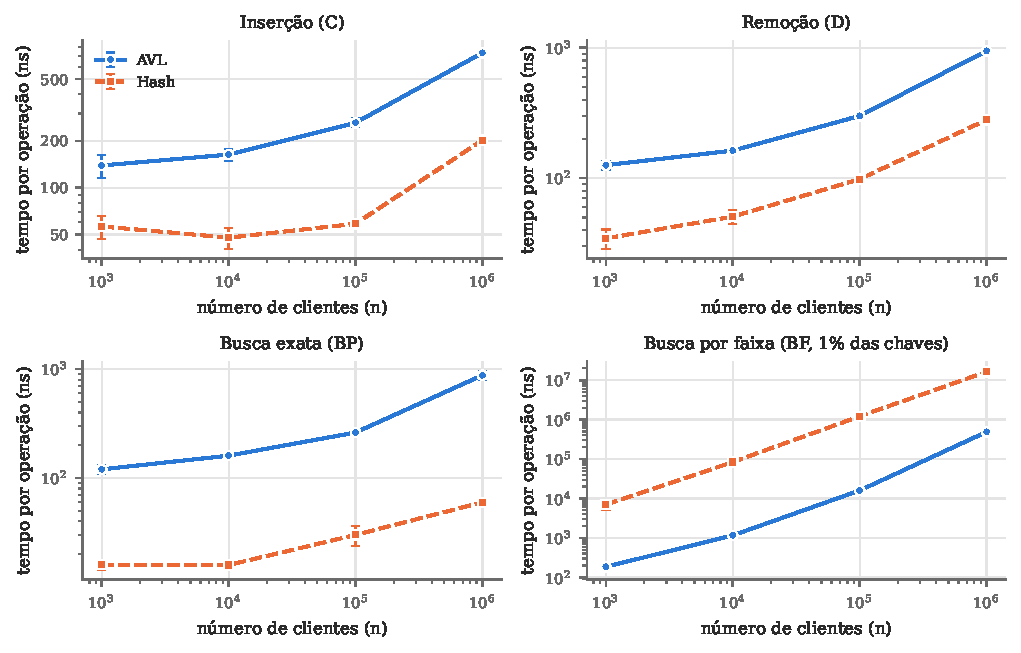
\includegraphics[width=0.85\textwidth]{figuras/exp1_tempo_por_operacao.pdf}
\caption{Experimento 1: tempo m\'edio por opera\c{c}\~ao em fun\c{c}\~ao do n\'umero de clientes (escalas logar\'itmicas). A hash vence inser\c{c}\~ao, remo\c{c}\~ao e \texttt{BP}; a AVL vence a \texttt{BF} por uma margem muito maior.}
\label{fig:exp1}
\end{figure*}

As duas estruturas n\~ao vencem nas mesmas opera\c{c}\~oes, como previsto pela an\'alise de complexidade. A hash \'e de 2,5 a 4,5 vezes mais r\'apida na inser\c{c}\~ao, de 3,1 a 3,6 vezes na remo\c{c}\~ao e de 7,5 a 14,7 vezes na \texttt{BP}: ela faz cerca de uma compara\c{c}\~ao de chave por opera\c{c}\~ao, enquanto a AVL faz de 10 a 20, aproximadamente $\log_2 n$. Na \texttt{BF}, a rela\c{c}\~ao se inverte com folga: a AVL \'e de 33 a 76 vezes mais r\'apida (por exemplo, 489\us\ contra 16,3\ms\ com $n = 10^6$), pois visita apenas os clientes da faixa e dois caminhos, enquanto a hash varre a tabela inteira e ainda ordena as entradas selecionadas.

A Tabela~\ref{tab:forma} mostra a forma das estruturas. A altura da AVL ficou entre o m\'inimo $\lceil\log_2(n+1)\rceil$ e bem abaixo do limite te\'orico de $1{,}44\log_2 n$ (24 contra 28,7 com $n = 10^6$). O n\'umero de rota\c{c}\~oes por opera\c{c}\~ao \'e praticamente constante em $n$: cerca de 0,70 por inser\c{c}\~ao e 0,37 por remo\c{c}\~ao. Na hash, cerca de 16\% das inser\c{c}\~oes criam uma entrada num balde j\'a ocupado (colis\~ao), mas a maior lista nunca passou de 2 entradas, o que confirma o bom espalhamento da fun\c{c}\~ao multiplicativa. As duas estruturas ocupam mem\'oria semelhante, cerca de 31\,MiB para $10^6$ clientes.

\begin{table}[t]
\centering
\small
\setlength{\tabcolsep}{3.5pt}
\begin{tabular}{rrrrrrr}
\toprule
$n$ & alt. & $1{,}44\log_2 n$ & rot./ins. & rot./rem. & colis\~oes & lista \\
\midrule
$10^3$ & 12 & 14,4 & 0,713 & 0,366 & 158 & 2 \\
$10^4$ & 16 & 19,1 & 0,702 & 0,369 & 1\,743 & 1 \\
$10^5$ & 20 & 23,9 & 0,701 & 0,373 & 16\,414 & 2 \\
$10^6$ & 24 & 28,7 & 0,705 & 0,373 & 165\,292 & 2 \\
\bottomrule
\end{tabular}
\caption{Experimento 1: altura e rota\c{c}\~oes da AVL; colis\~oes e maior lista de um balde na hash, ap\'os inserir $n$ clientes.}
\label{tab:forma}
\end{table}

\begin{figure}[t]
\centering
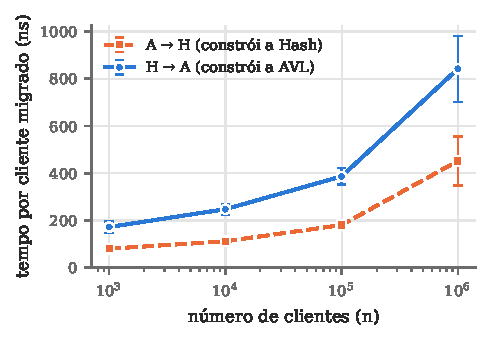
\includegraphics[width=0.9\columnwidth]{figuras/exp1_migracao.pdf}
\caption{Experimento 1: custo da migra\c{c}\~ao entre modos, por cliente migrado.}
\label{fig:migracao}
\end{figure}

O custo da pr\'opria migra\c{c}\~ao est\'a na Figura~\ref{fig:migracao}. Construir a AVL (H$\to$A) custa cerca do dobro de construir a hash (A$\to$H), em todos os tamanhos: com $10^6$ clientes, 0,84\,s contra 0,45\,s. Isso reflete a diferen\c{c}a entre $O(n\log n)$ e $O(n)$ e o fato de a listagem ordenada da AVL tornar cada inser\c{c}\~ao na hash um anexo no fim do vetor. Com $10^6$ clientes, uma migra\c{c}\~ao custa o equivalente a mais de mil \texttt{BF} no modo A ou a algumas dezenas no modo H, portanto s\'o compensa se a carga seguinte for longa.

\subsection{Experimento 2: rotatividade}

Para $n \in \{10^4, 10^5, 10^6\}$, o \'indice foi preenchido com $n$ clientes (sem medir) e, em seguida, foram medidas $n$ opera\c{c}\~oes em duas cargas: \emph{s\'o entradas}, com $n$ novas inser\c{c}\~oes, e \emph{entra e sai}, em que cada opera\c{c}\~ao \'e, com probabilidade 1/2, uma inser\c{c}\~ao ou a remo\c{c}\~ao de um cliente ativo sorteado, de modo que o tamanho fica em torno de $n$. O preenchimento garante que as duas cargas operem sobre estruturas de tamanho compar\'avel.

\begin{figure}[t]
\centering
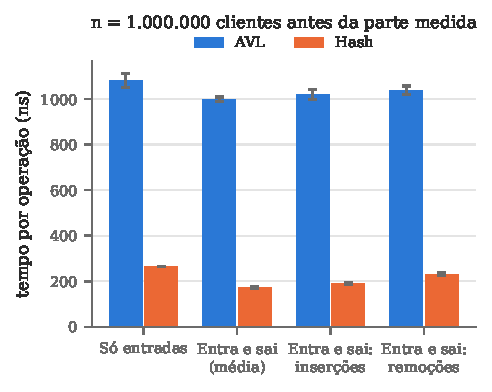
\includegraphics[width=0.9\columnwidth]{figuras/exp2_rotatividade_tempo.pdf}
\caption{Experimento 2: tempo por opera\c{c}\~ao nas duas cargas. As barras ``inser\c{c}\~oes'' e ``remo\c{c}\~oes'' foram medidas opera\c{c}\~ao a opera\c{c}\~ao e incluem o custo do rel\'ogio.}
\label{fig:exp2}
\end{figure}

A Figura~\ref{fig:exp2} mostra que intercalar entradas e sa\'idas n\~ao piora nenhuma das estruturas quando os poderes s\~ao quase todos distintos. Na AVL, a altura se manteve em 24 durante toda a carga \emph{entra e sai} (chegou a 25 com $2\cdot10^6$ clientes na carga \emph{s\'o entradas}), porque as remo\c{c}\~oes tamb\'em rebalanceiam; foram 0,36 rota\c{c}\~ao e 19,3 compara\c{c}\~oes por remo\c{c}\~ao. Na hash, a tabela n\~ao encolhe quando clientes saem: o fator de carga diminui, as listas ficam ainda mais curtas e a carga \emph{entra e sai} chega a ser mais r\'apida (173 contra 264\ns\ com $n = 10^6$), pois a carga \emph{s\'o entradas} tamb\'em paga os rehashes. Nessa distribui\c{c}\~ao, a remo\c{c}\~ao na hash \'e 4,5 vezes mais r\'apida que na AVL, raz\~ao parecida com a da inser\c{c}\~ao. A grande diverg\^encia da remo\c{c}\~ao aparece quando muitos clientes compartilham o mesmo poder, o que \'e medido no Experimento~5.

\subsection{Experimento 3: perfis de carga}

O sistema completo foi iniciado com 20\,000 clientes (poder uniforme em $[0, 10^5)$), 20\,000 regi\~oes e 10\,000 rotas aleat\'orias. Depois foram medidos 50\,000 comandos sorteados com as propor\c{c}\~oes de dois perfis: \emph{predom\'inio de atualiza\c{c}\~oes} (\texttt{C} 30\%, \texttt{D} 25\%, \texttt{F} 20\%, e 5\% para cada um de \texttt{Z}, \texttt{T}, \texttt{BP}, \texttt{BF} e \texttt{CC}) e \emph{predom\'inio de consultas} (\texttt{BP} 30\%, \texttt{BF} 25\%, \texttt{CC} 30\%, \texttt{C} 5\%, \texttt{D} 4\%, \texttt{F} 3\%, \texttt{T} 2\%, \texttt{Z} 1\%). A largura da \texttt{BF} \'e 1\% do intervalo de poderes. A carga respeita as regras da entrada: clientes de identificador par nunca s\~ao encerrados e podem entrar na fila, e clientes de identificador \'impar podem ser encerrados e nunca entram na fila. Os mesmos comandos foram executados nos modos A e H.

\begin{figure}[t]
\centering
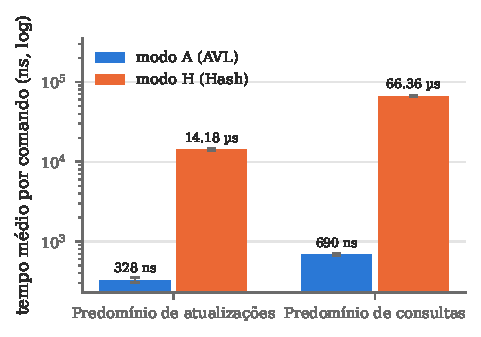
\includegraphics[width=0.9\columnwidth]{figuras/exp3_perfis_total.pdf}
\caption{Experimento 3: tempo m\'edio por comando em cada perfil e modo.}
\label{fig:exp3}
\end{figure}

\begin{figure*}[t]
\centering
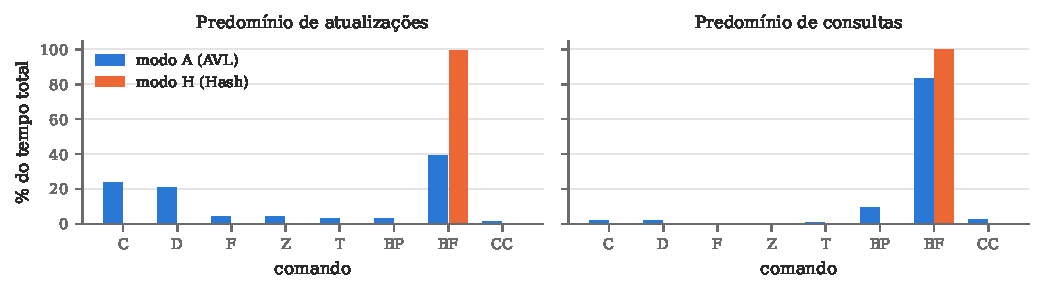
\includegraphics[width=0.85\textwidth]{figuras/exp3_parcela_por_comando.pdf}
\caption{Experimento 3: parcela do tempo total gasta em cada comando. No modo H, a \texttt{BF} responde por mais de 99\% do tempo nos dois perfis.}
\label{fig:exp3parcela}
\end{figure*}

O modo A foi 43 vezes mais r\'apido no perfil de atualiza\c{c}\~oes (328\ns\ contra 14,2\us\ por comando) e 96 vezes no perfil de consultas (690\ns\ contra 66,4\us) (Figura~\ref{fig:exp3}). A Figura~\ref{fig:exp3parcela} explica o resultado: no modo H, a \texttt{BF} consome mais de 99\% do tempo nos dois perfis, mesmo quando representa apenas 5\% dos comandos, porque cada uma custa cerca de 270\us, contra 2,6\us\ no modo A. Sem as \texttt{BF}, o modo H seria o mais r\'apido: no perfil de atualiza\c{c}\~oes, os demais comandos custaram em m\'edia 124\ns\ no modo H e 220\ns\ no modo A, principalmente gra\c{c}as a \texttt{C}, \texttt{D} e \texttt{BP}. Igualando a economia de cerca de 96\ns\ por comando com o custo extra de cerca de 270\us\ por \texttt{BF}, o modo H s\'o compensaria, neste cen\'ario, com menos de uma \texttt{BF} a cada 2\,800 comandos. Os comandos que n\~ao usam o \'indice (\texttt{F}, \texttt{Z}, \texttt{T}, \texttt{CC}) n\~ao dependem do modo, e as pequenas diferen\c{c}as observadas neles s\~ao provavelmente efeito do estado da cache, que a varredura da \texttt{BF} no modo H polui.

\subsection{Experimento 4: conjuntos disjuntos contra BFS}

Foram gerados mapas com $V \in \{10^3, 10^4, 10^5\}$ regi\~oes e grau m\'edio $g \in \{0{,}5;\ 1;\ 2;\ 4;\ 16\}$, isto \'e, $E = gV/2$ rotas aleat\'orias sem la\c{c}os nem repeti\c{c}\~oes. A constru\c{c}\~ao foi medida por elemento (regi\~ao ou rota): para os conjuntos disjuntos, \texttt{criar} e \texttt{unir}; para a BFS, a montagem das listas de adjac\^encia de que ela precisa. As consultas usam os mesmos pares aleat\'orios nos dois m\'etodos: 100\,000 para os conjuntos disjuntos e $2\cdot10^7/(V + 2E)$ (limitado a $[20, 2000]$) para a BFS.

\begin{figure*}[t]
\centering
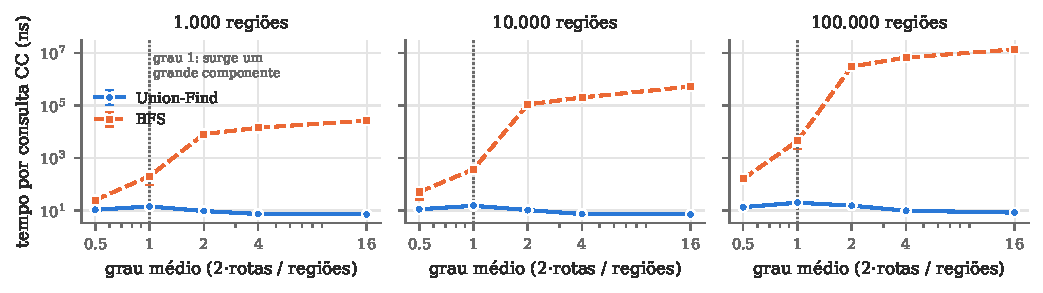
\includegraphics[width=0.85\textwidth]{figuras/exp4_consulta.pdf}
\caption{Experimento 4: tempo por consulta \texttt{CC}. A linha pontilhada marca o grau m\'edio 1, a partir do qual surge um componente gigante.}
\label{fig:exp4}
\end{figure*}

\begin{figure}[t]
\centering
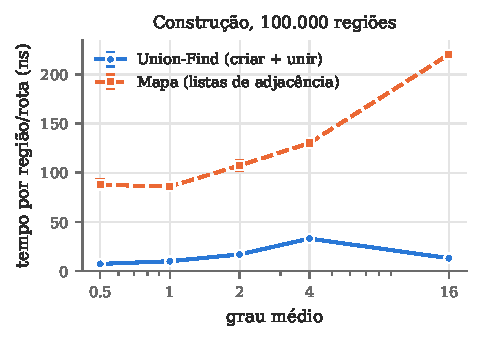
\includegraphics[width=0.9\columnwidth]{figuras/exp4_construcao.pdf}
\caption{Experimento 4: custo de constru\c{c}\~ao por regi\~ao ou rota, com $10^5$ regi\~oes.}
\label{fig:exp4construcao}
\end{figure}

Os conjuntos disjuntos responderam cada consulta em 7 a 20\ns, independentemente do tamanho e da densidade do mapa (Figura~\ref{fig:exp4}): com compress\~ao de caminho, cada busca de representante percorreu em m\'edia no m\'aximo um passo, e cada consulta, no m\'aximo 2. O custo da BFS depende da estrutura do grafo. Abaixo do grau 1, quase todos os componentes s\~ao pequenos e a busca termina cedo (25 a 161\ns). Acima dele, surge um componente gigante \citep{erdos1960}: a fra\c{c}\~ao de pares conectados observada (63\% com $g=2$ e 96\% com $g=4$) coincide com o quadrado da fra\c{c}\~ao de regi\~oes no componente gigante prevista pela teoria (0,80 e 0,98). A BFS passa ent\~ao a visitar dezenas de milhares de regi\~oes por consulta, cerca de metade do componente at\'e achar o destino, e chega a 13,8\ms\ com $10^5$ regi\~oes e grau 16, quase seis ordens de grandeza acima dos conjuntos disjuntos.

Na constru\c{c}\~ao (Figura~\ref{fig:exp4construcao}), os conjuntos disjuntos tamb\'em s\~ao mais baratos (6 a 33\ns\ por elemento, contra 31 a 220\ns\ para as listas de adjac\^encia, que alocam e redimensionam um vetor por regi\~ao) e ocupam muito menos mem\'oria (781\,KiB contra 31\,MiB com $10^5$ regi\~oes e grau 16). O Mapa continua necess\'ario porque guarda os nomes e as rotas com seus custos; para a pergunta \texttt{CC}, por\'em, os conjuntos disjuntos s\~ao a escolha certa em qualquer cen\'ario medido. A BFS s\'o seria necess\'aria se rotas pudessem ser removidas, o que a especifica\c{c}\~ao n\~ao prev\^e.

\subsection{Experimento 5: distribui\c{c}\~ao dos poderes e largura da faixa}

No Experimento 5a, $n = 50\,000$ clientes receberam poderes uniformes em $[0, D)$, com $D \in \{1, 10, \dots, 10^6\}$: quanto menor $D$, mais clientes por poder ($k_p \approx n/D$). Foram medidas a inser\c{c}\~ao, 1\,000 \texttt{BP} e a remo\c{c}\~ao em ordem aleat\'oria (Figura~\ref{fig:exp5a}).

\begin{figure*}[t]
\centering
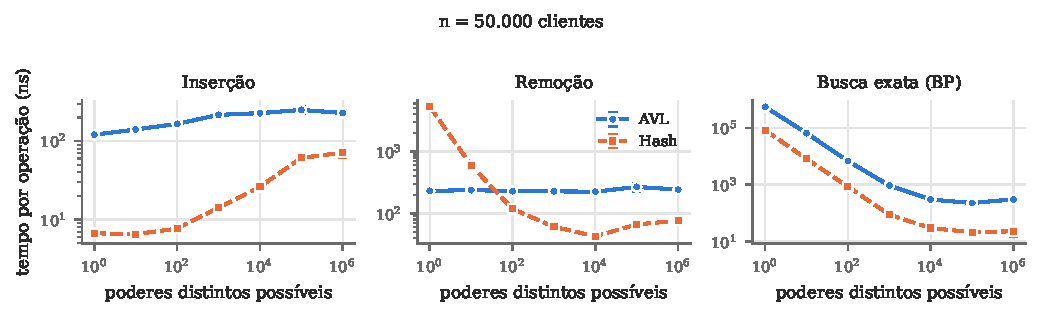
\includegraphics[width=0.85\textwidth]{figuras/exp5a_poderes_distintos.pdf}
\caption{Experimento 5a: efeito do n\'umero de poderes distintos poss\'iveis. Com poucos poderes, a remo\c{c}\~ao na hash fica at\'e 23 vezes mais lenta que na AVL.}
\label{fig:exp5a}
\end{figure*}

Este \'e o resultado em que as estruturas mais divergem. Na AVL, a remo\c{c}\~ao custou entre 228 e 269\ns\ para todo $D$, porque a chave composta torna todas as chaves distintas e a altura depende s\'o de $n$. Na hash, a remo\c{c}\~ao variou de 43\ns\ (5 clientes por poder) a 5,33\us\ com $D = 1$, em que todos os clientes est\~ao no mesmo vetor e cada remo\c{c}\~ao desloca em m\'edia cerca de 12\,500 identificadores. A invers\~ao ocorre entre 500 e 5\,000 clientes por poder. A inser\c{c}\~ao na hash, ao contr\'ario, fica \emph{mais barata} com poucos poderes (7\ns), porque o identificador \'e anexado ao fim de um vetor que est\'a na cache. Essa assimetria entre inser\c{c}\~ao e remo\c{c}\~ao \'e consequ\^encia direta da decis\~ao de agrupar os identificadores por poder. Na \texttt{BP}, as duas estruturas crescem com $k_p$, pois precisam devolver $k_p$ clientes, mas a hash \'e de 6 a 13 vezes mais r\'apida porque copia um vetor cont\'iguo, enquanto a AVL percorre $k_p$ n\'os.

\begin{figure}[t]
\centering
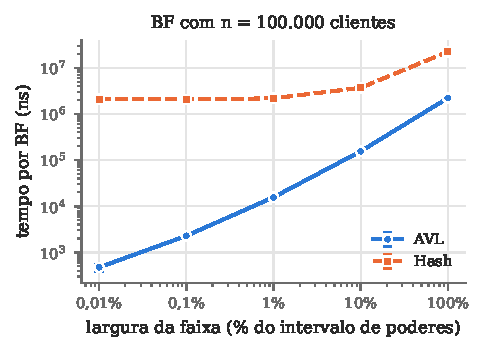
\includegraphics[width=0.9\columnwidth]{figuras/exp5b_largura_faixa.pdf}
\caption{Experimento 5b: tempo da \texttt{BF} em fun\c{c}\~ao da largura da faixa, com $n = 10^5$.}
\label{fig:exp5b}
\end{figure}

No Experimento 5b, com $n = 10^5$ clientes e poderes em $[0, 10^6)$, a largura da \texttt{BF} variou de 0,01\% a 100\% do intervalo (Figura~\ref{fig:exp5b}). O custo da AVL cresce linearmente com o n\'umero de clientes devolvidos, de 473\ns\ (10 clientes) a 2,2\ms\ (todos), confirmando o termo $O(\log n + m)$. O custo da hash fica praticamente constante em cerca de 2,1\ms\ at\'e 1\% de largura, o custo da varredura, e s\'o cresce quando a ordena\c{c}\~ao e a expans\~ao passam a dominar (22\ms\ com 100\%). A vantagem da AVL vai de 4\,400 vezes nas faixas mais estreitas a 10 vezes na faixa completa.

\subsection{Localidade de refer\^encia}

Os tempos medidos n\~ao s\~ao explicados apenas pelo n\'umero de compara\c{c}\~oes; o padr\~ao de acesso \`a mem\'oria tamb\'em pesa \citep{drepper2007}. Com $10^6$ clientes, cada estrutura ocupa cerca de 31\,MiB, cinco vezes a cache L3.

\paragraph{Descida na AVL.} Cada n\'o \'e alocado separadamente, e a descida \'e uma sequ\^encia de acessos indiretos a endere\c{c}os sem rela\c{c}\~ao entre si, em que o pr\'oximo endere\c{c}o s\'o \'e conhecido ap\'os a leitura do n\'o atual, o que impede a antecipa\c{c}\~ao pelo processador. Os n\'iveis mais altos da \'arvore s\~ao acessados em toda opera\c{c}\~ao e permanecem na cache, mas os n\'iveis mais baixos n\~ao cabem nela. Isso aparece claramente nos dados: de $n = 10^4$ (\'arvore de cerca de 600\,KiB, que cabe na L3) para $n = 10^6$, as compara\c{c}\~oes por inser\c{c}\~ao crescem apenas 1,5 vez (13,6 para 20,3), mas o tempo cresce 5 vezes (216\ns\ para 1,08\us). O custo por n\'ivel visitado passa de cerca de 16\ns\ para mais de 50\ns, valor t\'ipico de uma falha de cache que vai \`a mem\'oria principal.

\paragraph{Acesso na hash.} O vetor de baldes \'e cont\'iguo, mas o \'indice calculado pela fun\c{c}\~ao de espalhamento n\~ao tem rela\c{c}\~ao com o acesso anterior. Por isso, cada opera\c{c}\~ao tamb\'em falha na cache, tipicamente tr\^es vezes: no balde, no n\'o e no vetor de identificadores. O tempo da hash tamb\'em cresce com $n$ (a inser\c{c}\~ao passa de 22 para 264\ns), mas o n\'umero de falhas por opera\c{c}\~ao \'e constante, enquanto na AVL ele cresce com a altura. Isso explica por que a vantagem da hash na \texttt{BP} aumenta com $n$ (de 7,5 para 14,7 vezes).

\paragraph{Percursos.} O percurso de uma faixa na AVL visita n\'os logicamente vizinhos em sequ\^encia, e n\'os consecutivos compartilham quase todo o caminho at\'e a raiz, que j\'a est\'a na cache. Assim, cada cliente devolvido custa no m\'aximo cerca de uma falha (16 a 49\ns\ por cliente nas medi\c{c}\~oes). A varredura da \texttt{BF} na hash tem custo por n\'o semelhante (cerca de 20 a 26\ns, pois os n\'os das listas tamb\'em est\~ao espalhados), mas visita todos os $d$ n\'os em vez de apenas os $m$ da faixa, e \'e essa diferen\c{c}a algor\'itmica que produz as raz\~oes de 33 a 4\,400 vezes. O contraste mais claro de localidade est\'a no Experimento 5a: com $D = 1$, a \texttt{BP} na hash copia 50\,000 identificadores cont\'iguos em 83\us\ (1,7\ns\ cada), enquanto a AVL percorre 50\,000 n\'os em 555\us\ (11\ns\ cada). Da mesma forma, o deslocamento de cerca de 12\,500 inteiros na remo\c{c}\~ao da hash custa s\'o 5,3\us, menos de 0,5\ns\ por inteiro, porque \'e um acesso sequencial que o processador antecipa. Mesmo um algoritmo $O(k_p)$ pode ser r\'apido quando seus acessos s\~ao cont\'iguos, mas para $k_p$ grande ele ainda perde para o $O(\log n)$ da AVL.

%% =====================================================================
\section{Conclus\~ao}

Este trabalho implementou o sistema da Consultoria do Blibblon com seis TADs, incluindo um \'indice de clientes capaz de migrar, sem alterar o estado l\'ogico, entre uma \'arvore AVL e uma tabela hash. A implementa\c{c}\~ao produziu a sa\'ida esperada em todos os testes, incluindo o VPL, e a valida\c{c}\~ao com refer\^encia independente, verificador de invariantes e sanitizadores n\~ao encontrou erros.

As an\'alises te\'orica e experimental concordam: a hash vence as opera\c{c}\~oes pontuais por fatores de 2,5 a 15, e a AVL vence a busca por faixa por fatores de 10 a 4\,400, conforme a largura. Como uma \'unica \texttt{BF} na hash custa tanto quanto milhares de opera\c{c}\~oes pontuais, o modo A foi de 43 a 96 vezes mais r\'apido nos dois perfis de carga, e o modo H s\'o compensaria com menos de uma \texttt{BF} a cada cerca de 2\,800 comandos. A remo\c{c}\~ao \'e a opera\c{c}\~ao em que as estruturas mais divergem, e essa diverg\^encia depende da distribui\c{c}\~ao dos poderes: a AVL com chave composta n\~ao \'e afetada por poderes repetidos, enquanto na hash o custo cresce linearmente com o n\'umero de clientes por poder. Para a conectividade, os conjuntos disjuntos s\~ao melhores que a BFS na constru\c{c}\~ao, na consulta e na mem\'oria, em todos os mapas medidos.

Entre os aprendizados, destacam-se tr\^es. Primeiro, a escolha da chave (poder, identificador) na AVL resolveu de uma vez o desempate, a ordem da sa\'ida e o custo da remo\c{c}\~ao. Segundo, a nota\c{c}\~ao assint\'otica n\~ao basta para prever tempos: a localidade de refer\^encia explica por que a AVL piora mais que o n\'umero de compara\c{c}\~oes sugere e por que um deslocamento linear de inteiros cont\'iguos \'e t\~ao barato. Terceiro, medir corretamente exige cuidado com o que entra no la\c{c}o medido, como gerar a entrada antes e evitar aloca\c{c}\~oes desnecess\'arias. Como trabalho futuro, seria poss\'ivel tornar a remo\c{c}\~ao na hash independente de $k_p$ com uma estrutura ordenada por poder, ou fazer a tabela encolher ap\'os muitas remo\c{c}\~oes.

%% =====================================================================
\section{Agradecimentos e Declara\c{c}\~ao de Uso de IA Generativa}

Agrade\c{c}o aos professores e monitores da disciplina de Estruturas de Dados pelo material e pelo apoio.

Durante o desenvolvimento, foi utilizado o assistente Claude (Anthropic), por meio da ferramenta Claude Code, para: organizar o plano de trabalho em etapas; apoiar a implementa\c{c}\~ao e a revis\~ao dos TADs e do programa principal; escrever os testes de valida\c{c}\~ao, o programa de medi\c{c}\~ao e o script de gera\c{c}\~ao dos gr\'aficos; e redigir uma primeira vers\~ao deste texto a partir dos resultados obtidos. Todo o c\'odigo e todo o texto foram revisados pelo autor, que \'e integralmente respons\'avel pelo conte\'udo entregue.

%% =====================================================================
% Referencias escritas diretamente no formato que o aaai2026.bst produz
% (nao depende de rodar o BibTeX).
\begin{thebibliography}{9}
\providecommand{\natexlab}[1]{#1}

\bibitem[{Adelson-Velsky and Landis(1962)}]{adelson1962}
Adelson-Velsky, G.~M.; and Landis, E.~M. 1962.
\newblock An Algorithm for the Organization of Information.
\newblock \emph{Soviet Mathematics Doklady}, 3: 1259--1263.

\bibitem[{Cormen et~al.(2009)Cormen, Leiserson, Rivest, and Stein}]{cormen2009}
Cormen, T.~H.; Leiserson, C.~E.; Rivest, R.~L.; and Stein, C. 2009.
\newblock \emph{Introduction to Algorithms}.
\newblock Cambridge, MA: MIT Press, 3rd edition.

\bibitem[{Drepper(2007)}]{drepper2007}
Drepper, U. 2007.
\newblock What Every Programmer Should Know About Memory.
\newblock Red Hat, Inc. \url{https://people.freebsd.org/~lstewart/articles/cpumemory.pdf}.

\bibitem[{Erd{\H{o}}s and R{\'e}nyi(1960)}]{erdos1960}
Erd{\H{o}}s, P.; and R{\'e}nyi, A. 1960.
\newblock On the Evolution of Random Graphs.
\newblock \emph{Publications of the Mathematical Institute of the Hungarian Academy of Sciences}, 5: 17--61.

\bibitem[{Knuth(1998)}]{knuth1998}
Knuth, D.~E. 1998.
\newblock \emph{The Art of Computer Programming, Volume 3: Sorting and Searching}.
\newblock Reading, MA: Addison-Wesley, 2nd edition.

\bibitem[{Steele, Lea, and Flood(2014)}]{steele2014}
Steele, G.~L.; Lea, D.; and Flood, C.~H. 2014.
\newblock Fast Splittable Pseudorandom Number Generators.
\newblock In \emph{Proceedings of the 2014 ACM International Conference on Object Oriented Programming Systems Languages \& Applications (OOPSLA)}, 453--472.

\bibitem[{Tarjan(1975)}]{tarjan1975}
Tarjan, R.~E. 1975.
\newblock Efficiency of a Good But Not Linear Set Union Algorithm.
\newblock \emph{Journal of the ACM}, 22(2): 215--225.

\bibitem[{Williams(1964)}]{williams1964}
Williams, J. W.~J. 1964.
\newblock Algorithm 232: Heapsort.
\newblock \emph{Communications of the ACM}, 7(6): 347--348.

\bibitem[{Ziviani(2011)}]{ziviani2011}
Ziviani, N. 2011.
\newblock \emph{Projeto de Algoritmos com Implementa{\c{c}}{\~o}es em Pascal e C}.
\newblock S{\~a}o Paulo: Cengage Learning, 3rd edition.

\end{thebibliography}

\end{document}
